\chapter{Obstacle Experiments}
\label{chp:obstacle}

This chapter tests the central task of the thesis: reaching a beacon when an obstacle blocks the way. We first survey the real-room light field to confirm the obstacle leaves a navigable shadow. We then show the fused controller solving in simulation the scene that defeated both baselines. Next we fly the obstacle mission on the CrazyFlie. We close by reporting how the same board and controller carry over to a blimp.

\section{Experimental Setup}

We study the obstacle task in two stages, each isolating a different source of difficulty. We first repeat the simulation of Chapter~\ref{chp:algorithm}, the same scene in which the bearing-only and gradient-only baselines failed, and show that the fused controller succeeds where they did not. We then move to the real room, flying the CrazyFlie~2.1 with the photodiode board of Chapter~\ref{chp:hardware} and the full signal pipeline of Chapter~\ref{chp:realworld}, to confirm that the behaviour survives the ambient light, motor noise, and odometry drift of real flight. In both stages the obstacle is set into the route between the drone's start and the beacon, a little to one side rather than squarely in the line of sight. A box placed dead-centre would hide the beacon along the entire approach, reducing the task to a blind search. Offset to one side, it instead occludes the beacon over only part of the path while leaving a route the drone can discover, which is both the harder navigation problem and the more realistic one. The offset stays small enough that the drone must still steer around the box to reach the beacon.

The simulated scene is the one already shown in Figure~\ref{fig:sim-setup}, with the beacon, the obstacle pillar, and the drone approaching from one side, so we do not repeat it here. Figure~\ref{fig:obstacle-setup} shows the real-room geometry. The room carries the same two beacons as the open-space traverses of Chapter~\ref{chp:multibeacon}, and each obstacle flight targets one of them. The photograph in Figure~\ref{fig:flight-setup} shows the same box already in place. As in those traverses\todo{Its as a reader hard to see the link between the traverses of this chapter and the previous. So feel free to restate the full caviat of the geometry plot.}, the plotted positions are an indicative reference rather than a measured survey of the room.

\begin{figure}[h]
    \centering
    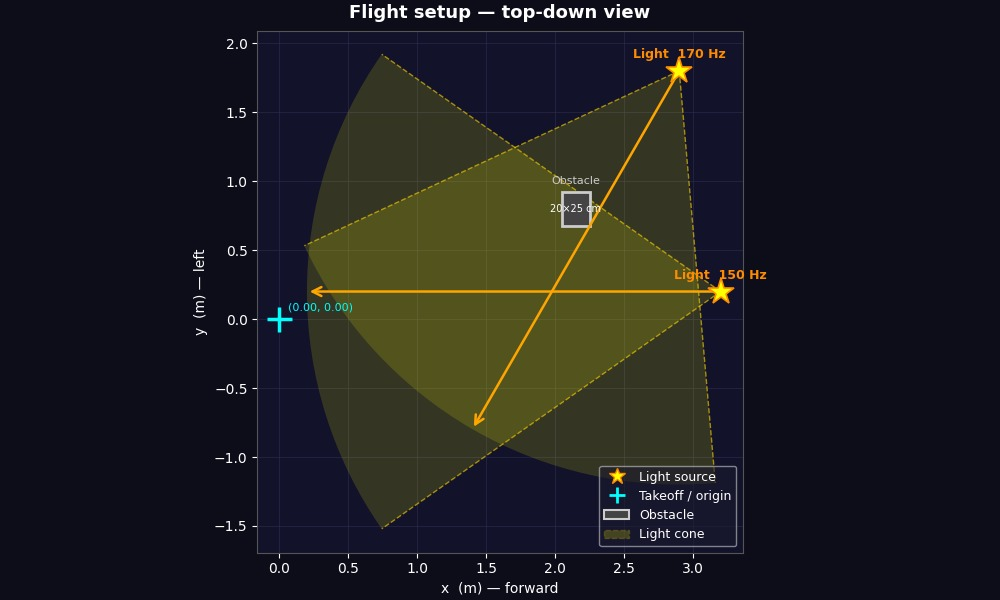
\includegraphics[width=0.6\textwidth]{figures/real_life_setup_plot_with_obstacle.jpeg}
    \caption{Top-down geometry of the real-room obstacle experiment. The room carries the same two beacons as the traverses of Chapter~\ref{chp:multibeacon}; each obstacle flight targets one of them, with the obstacle set into the route toward it and a little to one side. The layout is indicative rather than a precise survey of the room.}
    \label{fig:obstacle-setup}
\end{figure}

\section{SNR Field Mapping}
\label{sec:snr-field}

The fused controller relies on the light map precisely when the beacon is occluded, so before flying the obstacle mission we verify that the real-room SNR field behaves as the design assumes. Two properties must hold: the field must rise toward the beacon, so a gradient exists for the drone to climb, and the obstacle must leave a recognisable mark on it. We check both by surveying the field directly with a dedicated mapping flight, rather than inferring it from a navigation run.

We map the field with a survey flight that covers the area in a regular back-and-forth raster, a lawnmower pattern. The drone holds a fixed altitude of 0.8\,metres, the same height it uses during its navigation flights, so the survey samples the field the controller actually flies through. It moves at a slow, steady speed of about 0.2\,metres per second while logging the SNR at each photodiode, which yields a dense and even coverage of the area. The map records the field in 5\,centimetre cells over an area of about three by one and a half metres, a far denser and more even sampling than any single navigation flight builds. This gives four field maps in all: the two beacons, at 150 and 170\,Hz, each mapped with the obstacle in place and without it.

These maps must be read as a reference, not as a metric survey of the room. Their positions are localised by the drone's own odometry, which drifts over the course of a flight and depends strongly on the drone's starting angle. Even a small initial heading error shifts where the whole surveyed area lands, so the four maps cannot be laid directly on top of one another, and the distances within any one of them are not a true measurement of the room's geometry. What they do show, reliably, is how the SNR field behaves relative to the beacon, and that is all we ask of them. This\todo{What is "this" in this context?} is enough because the controller acts on a heading, not on an absolute beacon position. The algorithm of Chapter~\ref{chp:algorithm} is built around this, so drift in the odometry does not mislead it\todo{Why is this last sentence relevant.}.

Without the obstacle, the SNR field rises smoothly toward the beacon. As Figures~\ref{fig:snr-field-150} and~\ref{fig:snr-field-170} show, each beacon's field climbs from the far side of the room to a clear peak near the beacon, which confirms that the navigable gradient the controller depends on is present in the real room.

Placing the obstacle opens a region of low SNR behind it. Where the box stands between the survey and the beacon, the modulated signal can no longer reach the photodiodes directly, so the recovered SNR drops and leaves a shadow in the field. This shadow is the real-room counterpart of the occlusion the simulation creates with its pillar. It is precisely the region in which the bearing becomes unreliable and the drone must navigate on the stored map instead, the situation the recovering phase of Chapter~\ref{chp:algorithm} is designed to handle. In these survey maps the obstacle is drawn larger than the physical box, whose true size is shown later in the flight plots of Figure~\ref{fig:obstacle-good}. We enlarge it not only in the plots but in the drone's flight code, to leave a margin against odometry drift during the slow raster. The box itself is never bigger. Only the footprint the drone treats as off-limits is enlarged, so it stays clear of the real obstacle.

The 170\,Hz field also appears to carry a slight dip near the 150\,Hz beacon, in a spot where the smooth fall-off alone would lead us to expect a somewhat higher SNR. We read this tentatively as an effect of the 150\,Hz beacon: where that beacon is bright it may begin to saturate the photodiodes, flattening their response and lowering the recovered SNR across all frequencies, the 170\,Hz one included. The dip is faint, and the survey cannot separate it cleanly from the ordinary fall-off with distance, so we note it only as a likely trace of the same close-range saturation that bounds the sensor's operating range, and a reminder that the field is clean only in the band where the photodiodes are neither starved nor saturated.

\begin{figure}[h]
    \centering
    \subfigure[No obstacle]{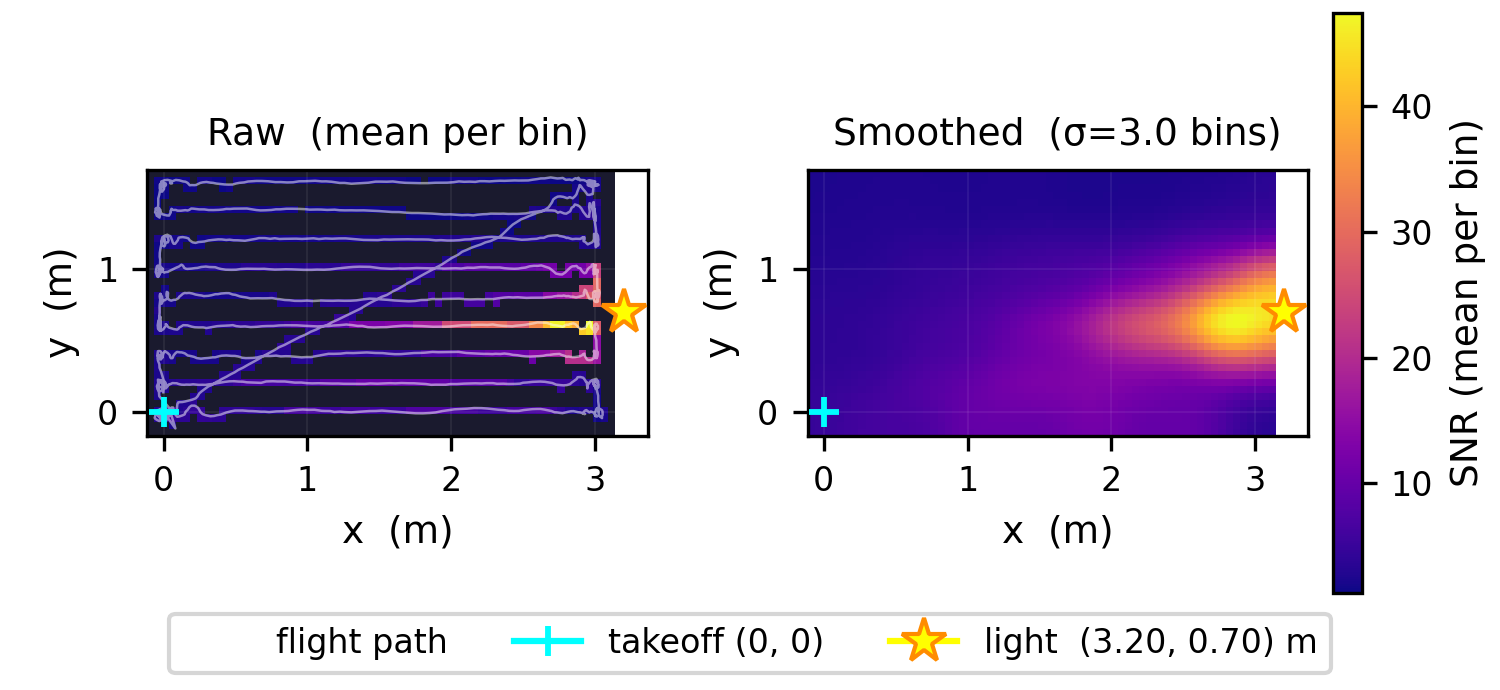
\includegraphics[width=\textwidth]{figures/real_data_gather_flights/150hz_lawnmower_no_obstacle.png}}\\
    \subfigure[With obstacle]{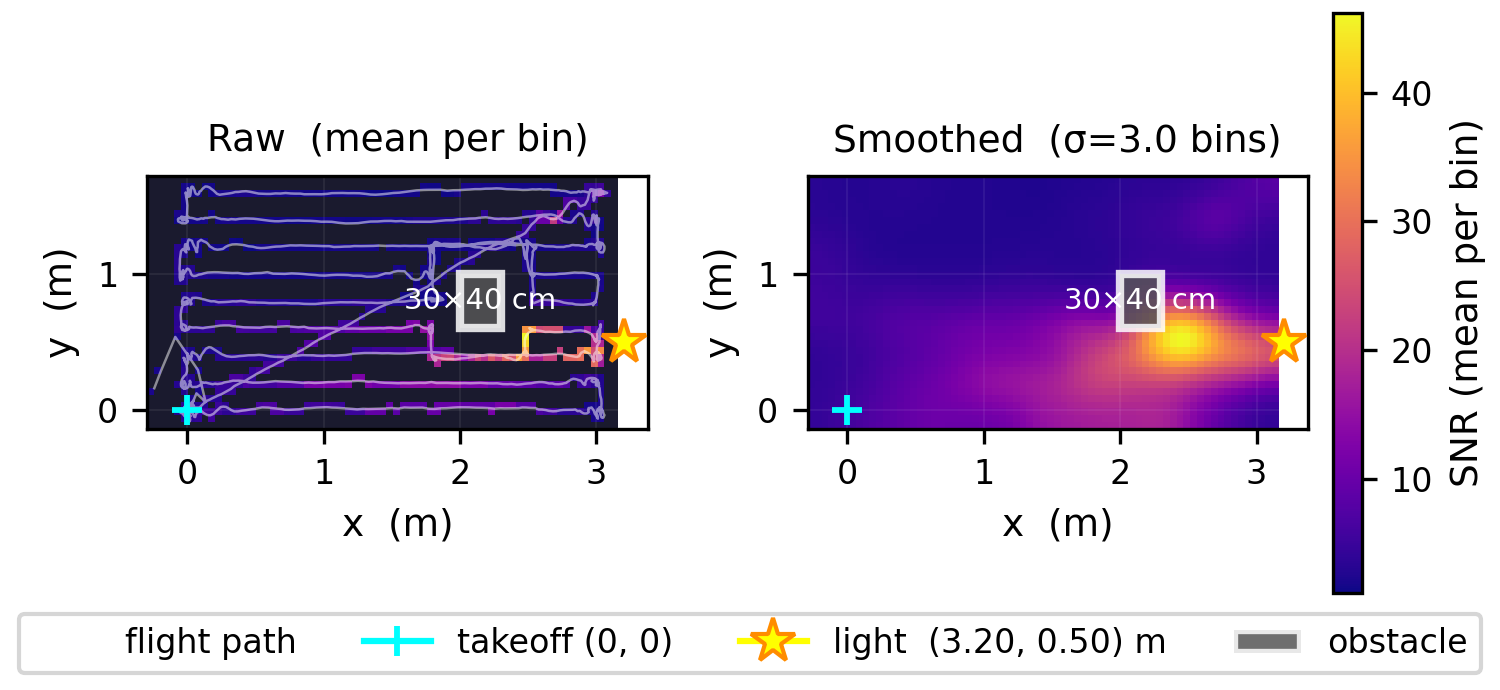
\includegraphics[width=\textwidth]{figures/real_data_gather_flights/150hz_lawnmower_with_obstacle.png}}
    \caption{SNR field of the real room for the 150\,Hz beacon, surveyed on a dense raster at a fixed altitude, without and with the obstacle. Each panel shows the raw per-cell mean alongside a smoothed version, with the flight path overlaid. Without the obstacle the field rises smoothly to a peak at the beacon; with the obstacle a low-SNR shadow opens behind the box. Positions are localised from odometry and serve as a reference, not a metric survey.}
    \label{fig:snr-field-150}
\end{figure}\todo{A small title above the figure showing that its the 150Hz figure would be nice. Also make sure to use separate labels for the subplots. Then also reference the subplots in the text. We should also more explicitly note that the SNR color grade goes from-to different numbers.}

\begin{figure}[h]
    \centering
    \subfigure[No obstacle]{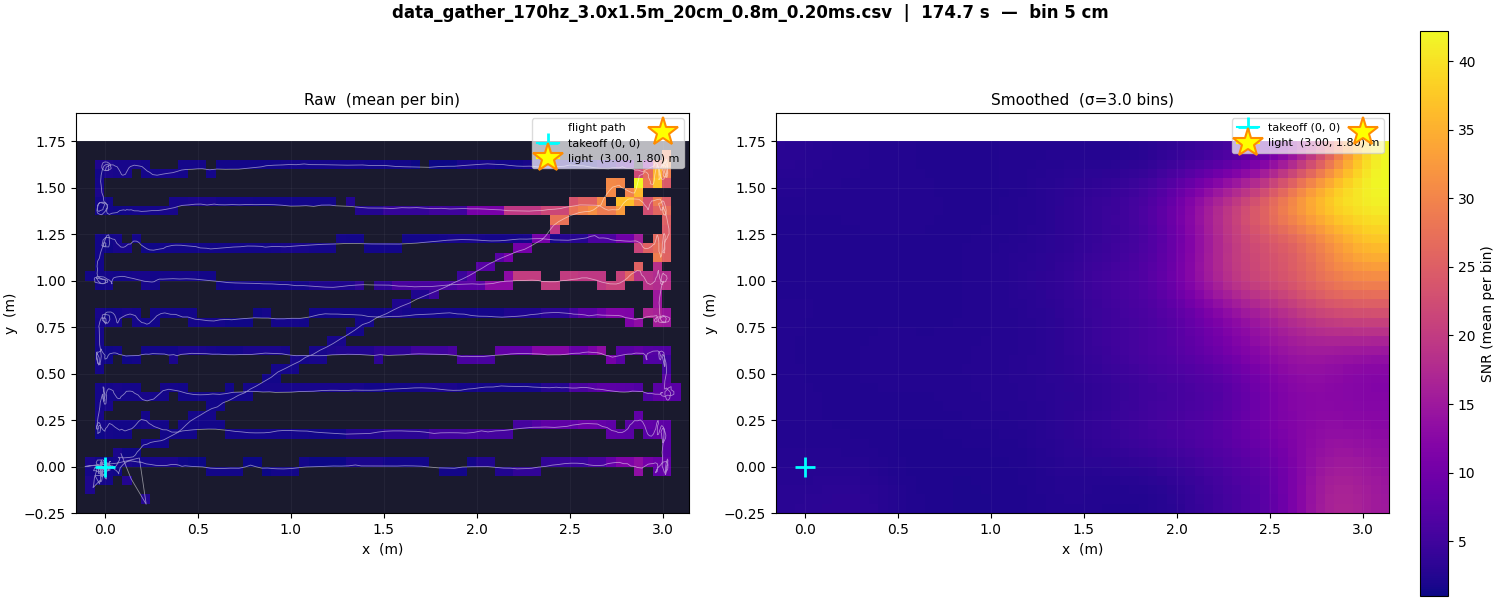
\includegraphics[width=\textwidth]{figures/real_data_gather_flights/170hz_lawnmower_no_obstacle.png}}\\
    \subfigure[With obstacle]{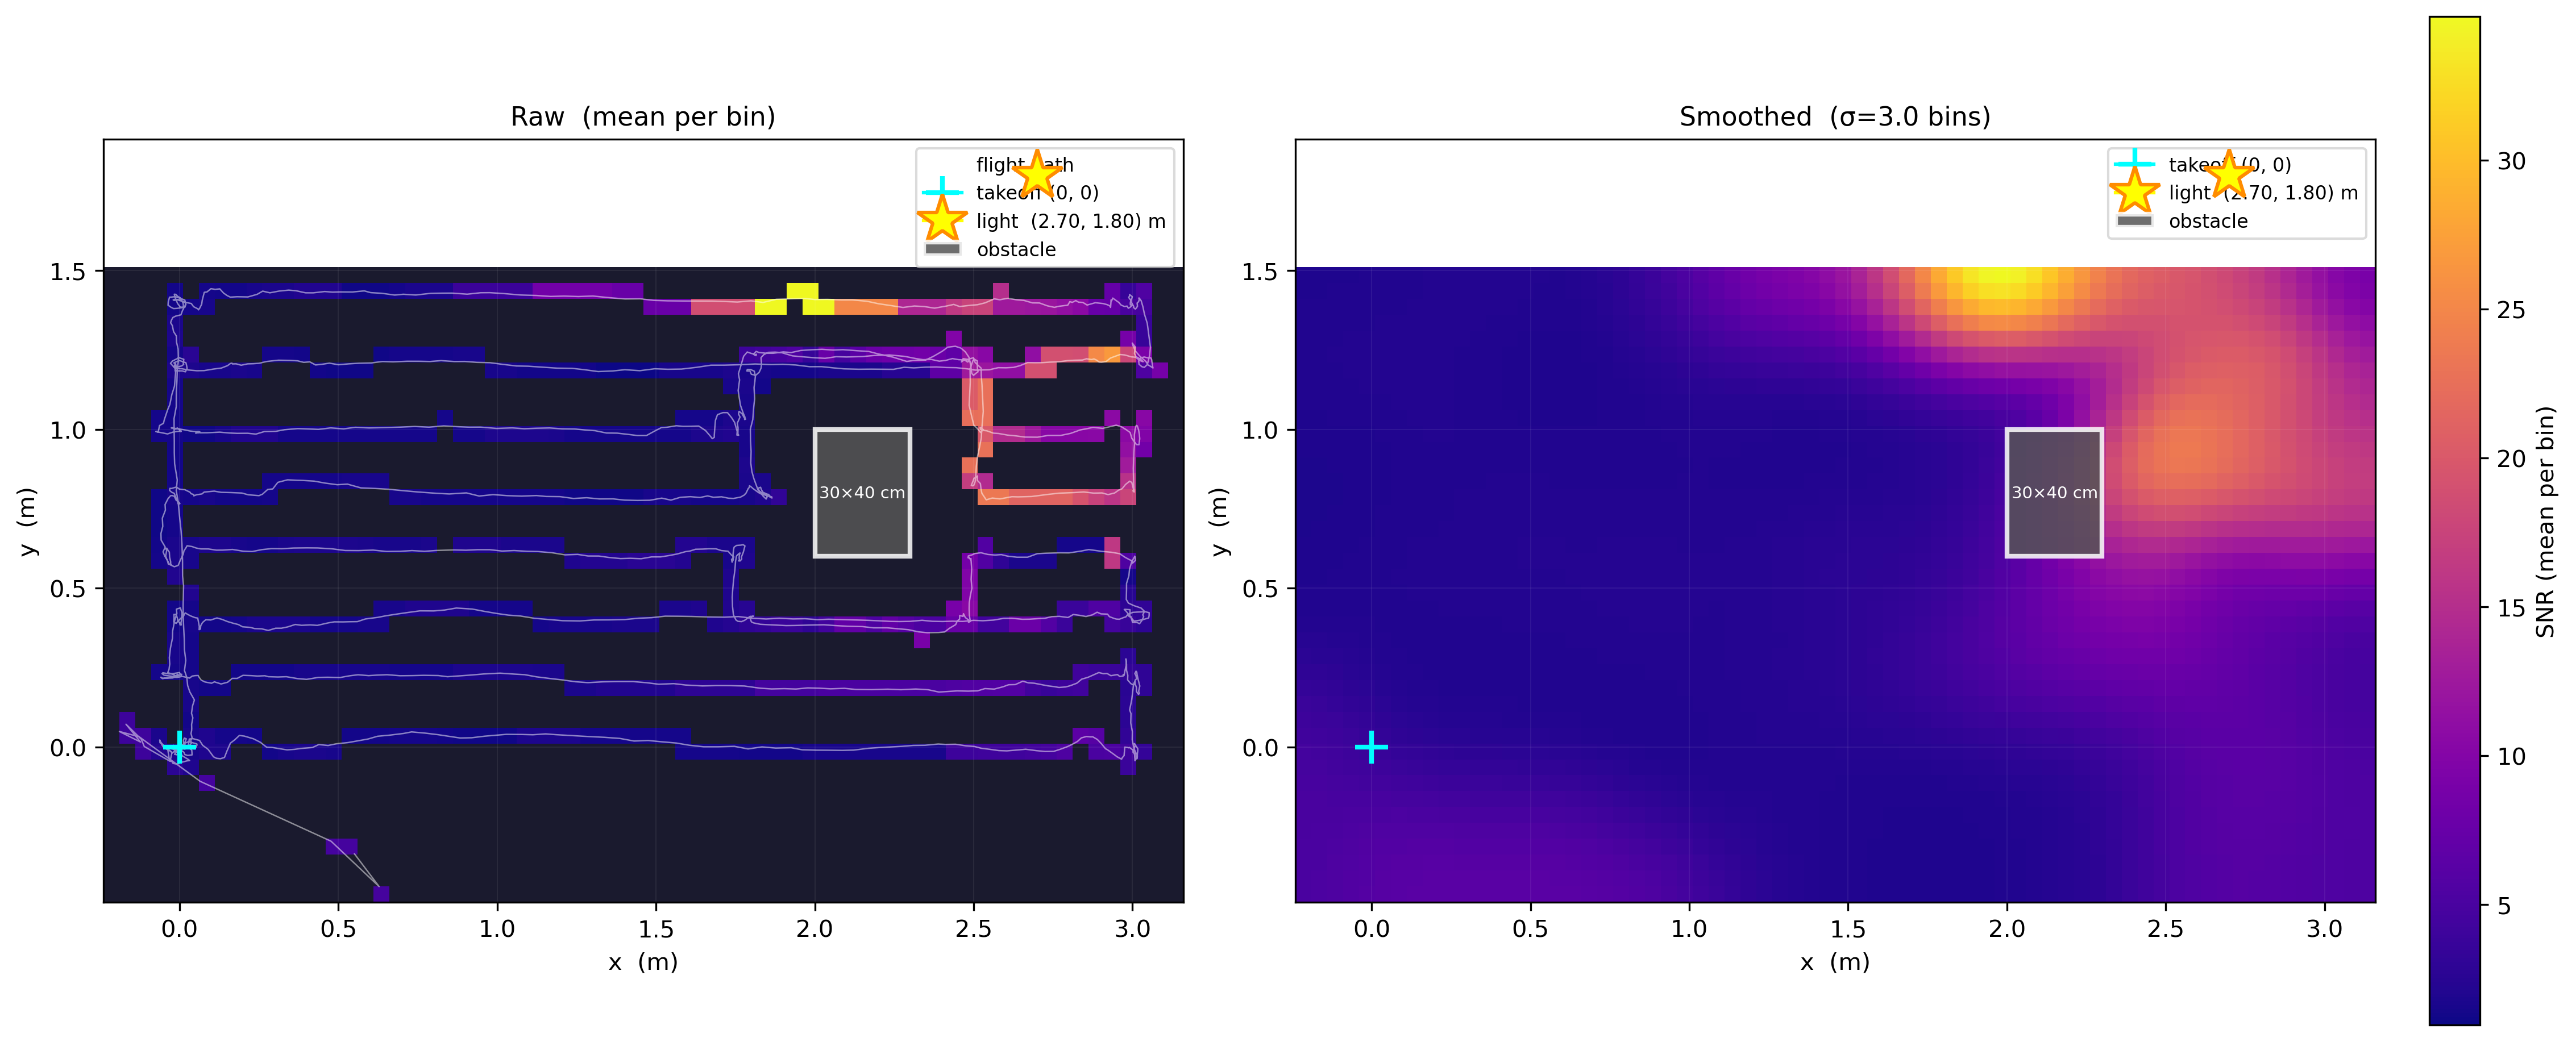
\includegraphics[width=\textwidth]{figures/real_data_gather_flights/170hz_lawnmower_with_obstacle.png}}
    \caption{SNR field of the real room for the 170\,Hz beacon, without and with the obstacle, in the same format as Figure~\ref{fig:snr-field-150}. The field again rises to a peak near the beacon and shows the obstacle's shadow. A slight dip also appears near the 150\,Hz beacon, which we tentatively attribute to that beacon saturating the photodiodes and lowering the recovered SNR across all frequencies.}
    \label{fig:snr-field-170}
\end{figure}

\section{Obstacle Avoidance}

\subsection{Simulation}

With the SNR field confirmed navigable, we turn to the avoidance task itself. In simulation the fused controller solves the task that defeated both baselines of Chapter~\ref{chp:algorithm}. Flying the same scene, from the same start toward the same beacon as the bearing-only and gradient-only runs, it routes cleanly around the obstacle and reaches the beacon, as Figure~\ref{fig:fused-sim} shows. After a brief opening segment on the bearing alone, while the map is still too sparse for a reliable gradient, the controller blends in the gradient and from then on steers by the combined bearing-and-gradient heading\todo{This sentence is overly long and should be split.}. This blended heading curves the path around the pillar on its own, so the drone neither flies into the obstacle nor has to stop and search. The avoidance here comes from the fusion of the two cues rather than from the recovering fallback, which this run never needs to enter, since the bearing remains valid throughout the curved approach. This contrast with the baselines \todo{Which baselines?} is the central result of the run: the bearing-only controller collides with the pillar in Figure~\ref{fig:bearing-fail} and the gradient-only controller stalls in Figure~\ref{fig:gradient-fail}, whereas the fused controller\todo{Is this not too much duplicate information?}, holding both the immediate bearing and a memory of the field, rounds the obstacle and arrives.

\begin{figure}[h]
    \centering
    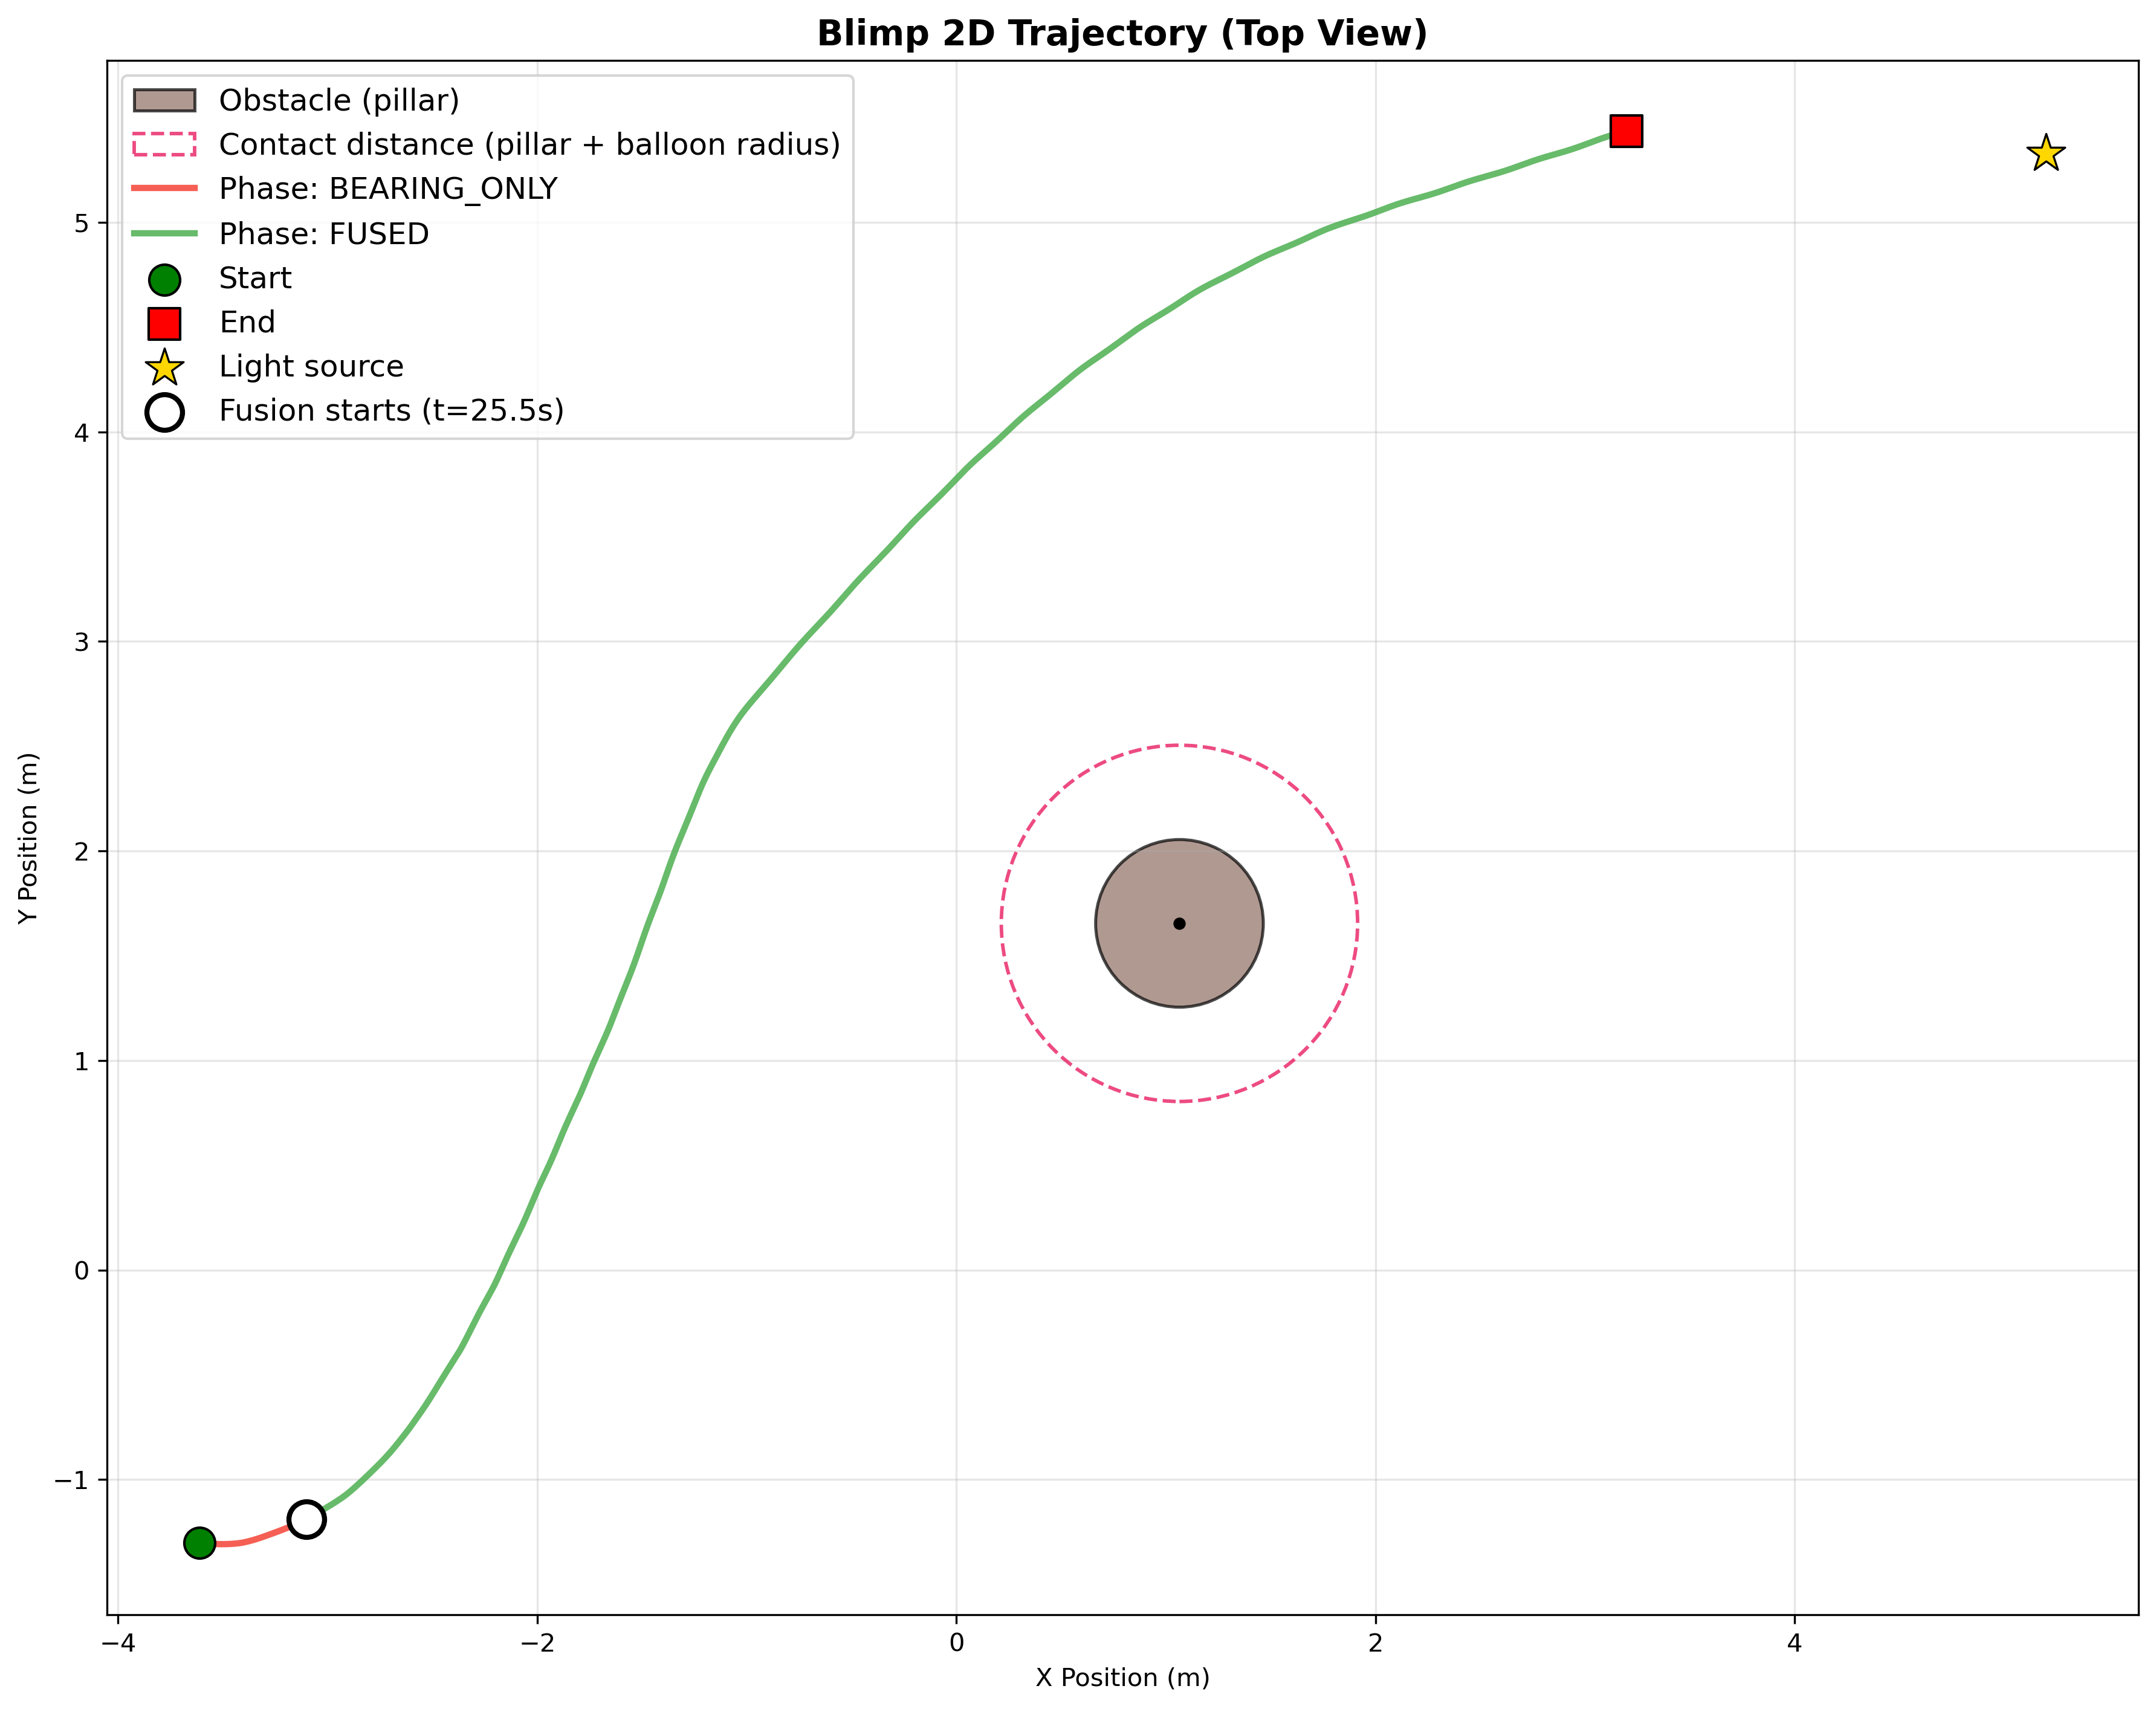
\includegraphics[width=0.6\textwidth]{figures/fused_sim/blimp_trajectory_2d.png}
    \caption{In simulation, the fused controller routes around the obstacle and reaches the beacon on the blended bearing-and-gradient heading, where the bearing-only and gradient-only controllers fail in Figures~\ref{fig:bearing-fail} and~\ref{fig:gradient-fail}.}
    \label{fig:fused-sim}
\end{figure}

\subsection{Real-World Flight}

Simulation removes the ambient light and motor noise of real flight, so we now fly the obstacle mission on the CrazyFlie to confirm the behaviour survives them\todo{Too coloquial and informal.}. The drone takes off from its origin and heads for a single beacon, with the box set into the route a little to one side of the straight-line path.

We present two runs that bring the drone close to the obstacle. We fly the mission several times, and the drone reaches the beacon on every run, but on many of them the path stays clear of the box, so the obstacle never comes into play. The two we show pass close to it, where the controller must contend with the obstacle, and they exercise it in two different ways.

In both flights the drone reaches the beacon, steering around the box rather than into it, and the controller registers its arrival and dwells. We do not run a controlled repeatability trial, so these results demonstrate that the avoidance works rather than measuring how reliably it succeeds.

In the first flight the beacon signal weakens enough that the controller falls back on the map, exercising the recovering phase that the simulation never needed. Figure~\ref{fig:obstacle-good} shows the result. The upper panel plots the path leaving the origin and steering past the box, drawn over the light map the drone builds as it flies, whose cells are coloured by the SNR measured there. The lower panel tracks the controller's state and the overall SNR over time. The flight walks the state machine of Chapter~\ref{chp:algorithm} through searching, aligning, and approaching, and then, as the drone passes behind the obstacle, into recovering and back. As it moves behind the box the beacon is occluded, the overall SNR falls to a trough\todo{Colloquial -- and this sentence is a bit long. Maybe split.}, and the magnitude of the bearing estimate drops below its trust threshold, so the bearing no longer yields a usable heading. This is exactly the situation a purely reactive controller cannot handle: with no memory of the field it would have no direction left to follow. The stored map supplies one. Because the gradient fitted to the map still meets its reliability conditions, the state machine enters recovering and the drone continues on the gradient direction alone, climbing the stored field to move out of the obstacle's shadow. As soon as the bearing rises back above its trust threshold the controller returns to approaching, closes on the beacon, and dwells.

\begin{figure}[h]
    \centering
    \subfigure[Flight path over the light map the drone built]{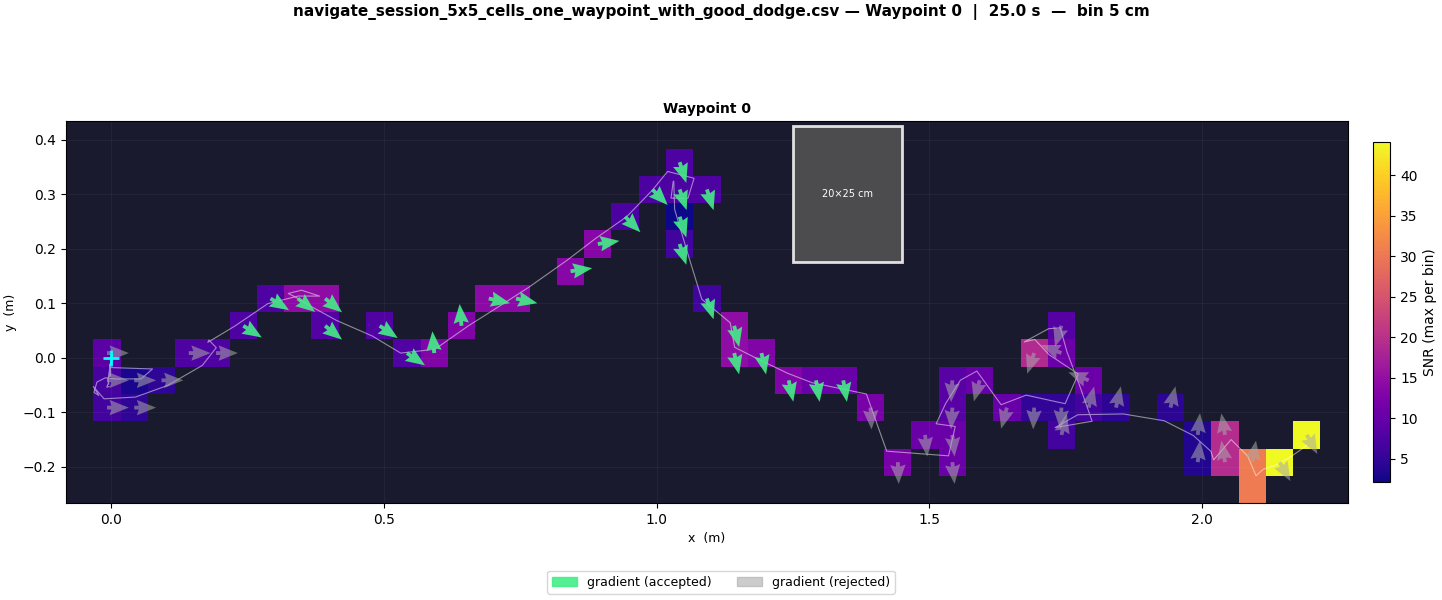
\includegraphics[width=0.85\textwidth]{figures/obstacle_dodging_real/one_waypoint_good_dodge_trajectory.png}}\\
    \subfigure[Controller state and overall SNR over time]{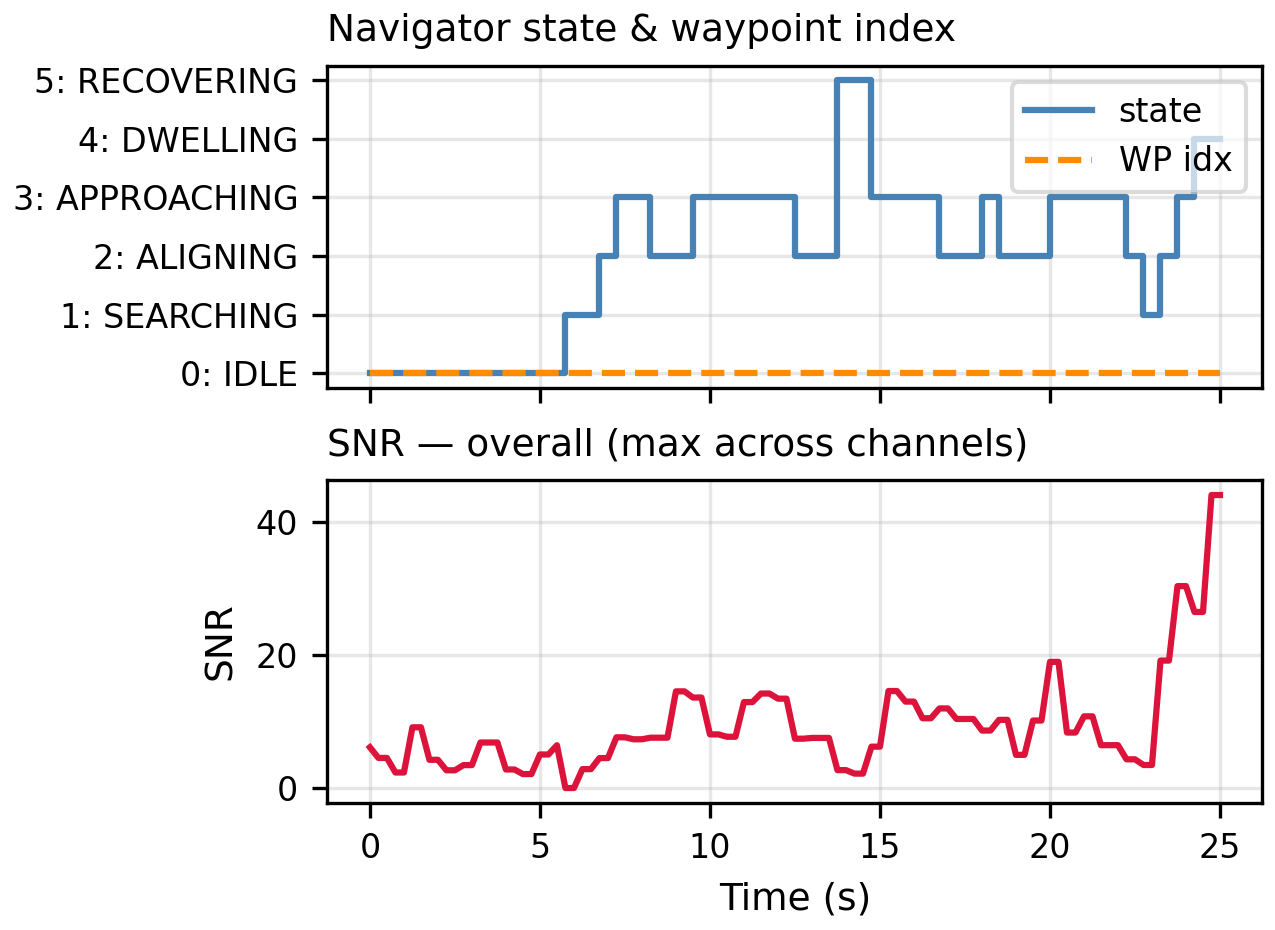
\includegraphics[width=0.85\textwidth]{figures/obstacle_dodging_real/one_waypoint_good_dodge_state_snr.png}}
    \caption{Real-world obstacle flight on the CrazyFlie~2.1. The drone steers around the box to reach the beacon; as it rounds the obstacle the SNR falls and the bearing becomes unreliable, so the state machine enters the recovering phase and follows the gradient map alone until the signal comes back.}
    \label{fig:obstacle-good}
\end{figure}

The second flight reaches the beacon without ever falling back on the map alone, and so represents the other operating regime. The difference between the two flights is geometric rather than a change in the controller: the first passes through more of the box's shadow, where the beacon is occluded and the bearing is lost, whereas the second skirts the shadow's edge. The drone therefore keeps a usable bearing throughout, so the controller stays in its approaching phase and never enters recovering. The blended bearing-and-gradient heading alone is enough to steer the path around the obstacle, as Figure~\ref{fig:obstacle-dodge} shows. Taken together, the two flights show the controller drawing on the map only as far as each situation requires: recovering on the gradient when the bearing drops below its trust threshold, and rounding the obstacle on the fused heading when it does not.

\begin{figure}[h]
    \centering
    \subfigure[Flight path over the light map the drone built]{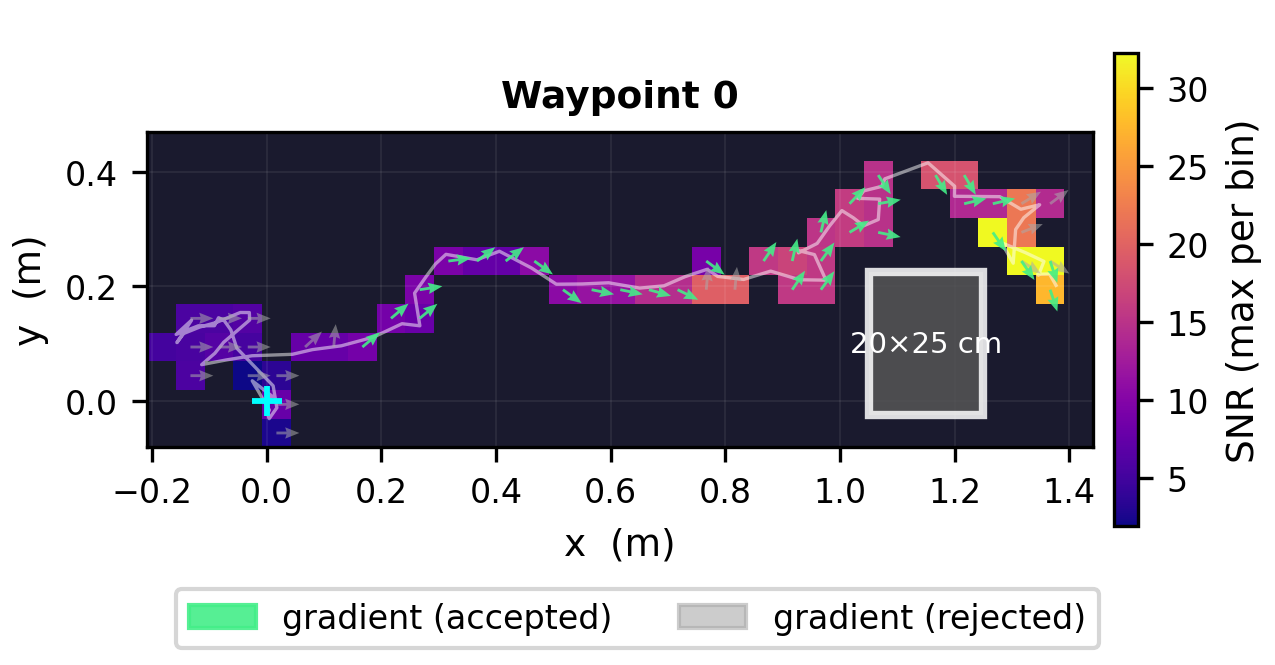
\includegraphics[width=0.85\textwidth]{figures/obstacle_dodging_real/one_waypoint_dodges_obstacle_trajectory.png}}\\
    \subfigure[Controller state and overall SNR over time]{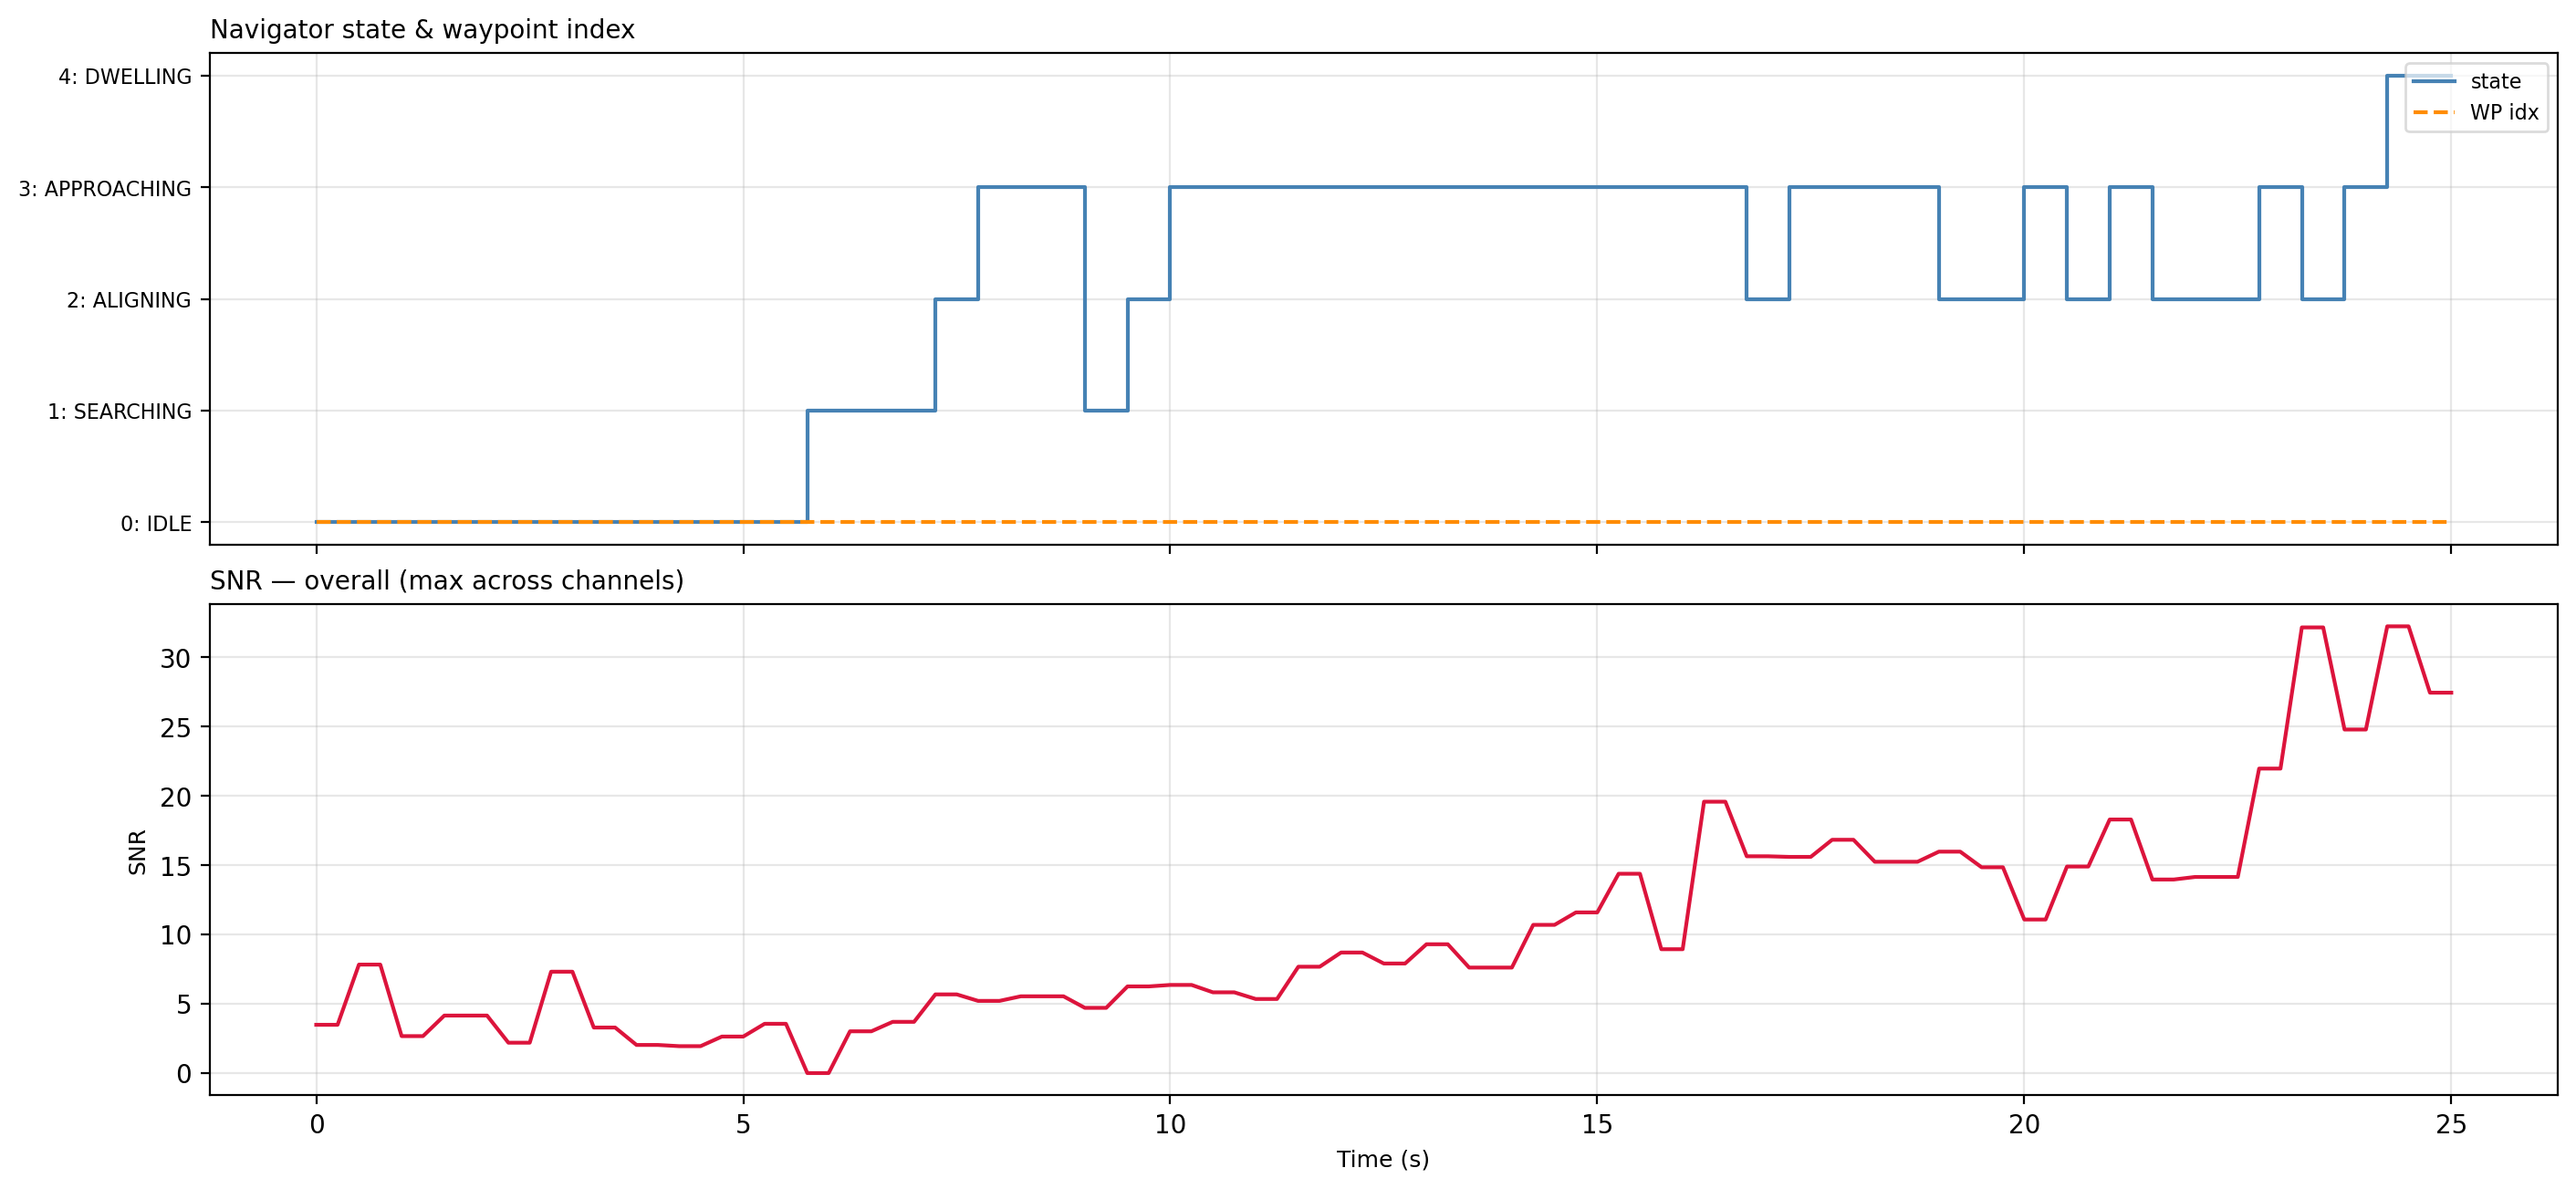
\includegraphics[width=0.85\textwidth]{figures/obstacle_dodging_real/one_waypoint_dodges_obstacle_state_snr.png}}
    \caption{A second real-world obstacle flight in which the drone keeps a usable bearing throughout, so the controller stays in its approaching phase and steers around the box on the blended heading without ever entering the recovering phase.}
    \label{fig:obstacle-dodge}
\end{figure}

\section{Generalisation to a Blimp Platform}

Our own validation spans the Webots simulation and the CrazyFlie~2.1, but the contribution is not tied to that platform. We show this through a collaboration with Huang et al.~\cite{huang2026lta}, who developed the lighter-than-air blimp and the Webots simulation this thesis builds on. The blimp is a closely related micro-drone, held aloft by a helium balloon and driven by a different motor layout. The base bearing and single-photodiode gradient methods of Huang et al. were demonstrated on this blimp only in simulation, never flown on the real airframe~\cite{huang2026lta}. The real blimp flights instead use the contribution of this thesis. We develop the fused controller within the simulation, build the photodiode board of Chapter~\ref{chp:hardware}, and run the real-world experiments of this thesis on the CrazyFlie \todo{Why is this sentence here? Feels superfuous.}. Huang et al. then mounts the same board and fused controller on the real blimp, adapting only the low-level control to its motor layout, and confirms that it reaches several modulated beacons in turn and avoids obstacles there \todo{What is this "there"}, as it does on the CrazyFlie~\cite{huang2026lta}. The same board and algorithm therefore work across two different airframes, which shows that the approach depends on the light sensing rather than on the specifics of the platform.

The blimp flights also show a higher SNR than we obtain on the CrazyFlie. The photodiode board is the same and sits in the same place on both airframes, since the blimp is in essence\todo{colloquial.} a CrazyFlie with a different motor layout and a helium balloon on top. What differs is the motors: a buoyant platform stays aloft without constantly driving the motors, so on the blimp they run only when it moves and at far lower power.

\subsection{Motor Noise on the CrazyFlie}

The higher SNR on the blimp points to the motors as the likely cause, so we measure their effect directly on the CrazyFlie. We hold the board at a fixed pose and record the SNR while running an increasing number of its motors, both with the hardware anti-alias filter and without. Table~\ref{tab:motor-noise} and Figure~\ref{fig:motor-noise} show the result. The SNR falls steadily as more motors spin. With the hardware filter in place it drops from about 61 with all motors off to about 25 at full throttle, which confirms the motors are the dominant disturbance.

A motor couples noise into the board in two ways: it draws current that interferes electrically, and it shakes the board mechanically. To separate the two, we repeat the four-motor case with the motors moved onto extension wires, which isolates them mechanically while leaving them electrically connected. With the filter in place this recovers about half of the lost SNR, from about 25 back to about 43. Vibration and electrical interference therefore contribute in roughly equal measure, once the filter has dealt with the worst of the aliased noise.

The motors are therefore the main reason the CrazyFlie sees a lower SNR than the blimp. Because the blimp drives its motors far less, it avoids most of this penalty\todo{What penalty?}, which explains its higher SNR and the longer sensing range that comes with it\todo{Where does this longer sensing range come from? Did we already explain the relation to higher SNR and more range in a different chapter? Otherwise maybe leave it out.}. What this extra range could buy, and how a future board might suppress the mechanical half of the loss, we take up in Chapter~\ref{chp:futurework}.\todo{The future work forward reference is maybe not needed.}

\begin{table}[ht]
    \centering
    \caption{Overall SNR on the CrazyFlie at a fixed pose while running an increasing number of its motors, with the hardware anti-alias filter left unpopulated and with it soldered. Each cell is the mean $\pm$ standard deviation. The last row repeats the four-motor case with the motors moved onto extension wires, mechanically isolating them from the board.}
    \label{tab:motor-noise}
    \begin{tabular}{l c c}
        \hline
        Configuration & No HW filter & HW filter \\
        \hline
        0 motors                & $26.7 \pm 1.8$  & $60.6 \pm 16.3$ \\
        1 motor                 & $24.2 \pm 1.8$  & $49.2 \pm 10.9$ \\
        2 motors                & $23.2 \pm 1.7$  & $46.0 \pm 9.0$  \\
        3 motors                & $18.0 \pm 2.3$  & $28.7 \pm 3.2$  \\
        4 motors                & $16.7 \pm 2.2$  & $24.8 \pm 2.6$  \\
        \hline
        4 motors, extension wires & $19.3 \pm 1.5$ & $43.1 \pm 7.3$ \\
        \hline
    \end{tabular}
\end{table}

\begin{figure}[ht]
    \centering
    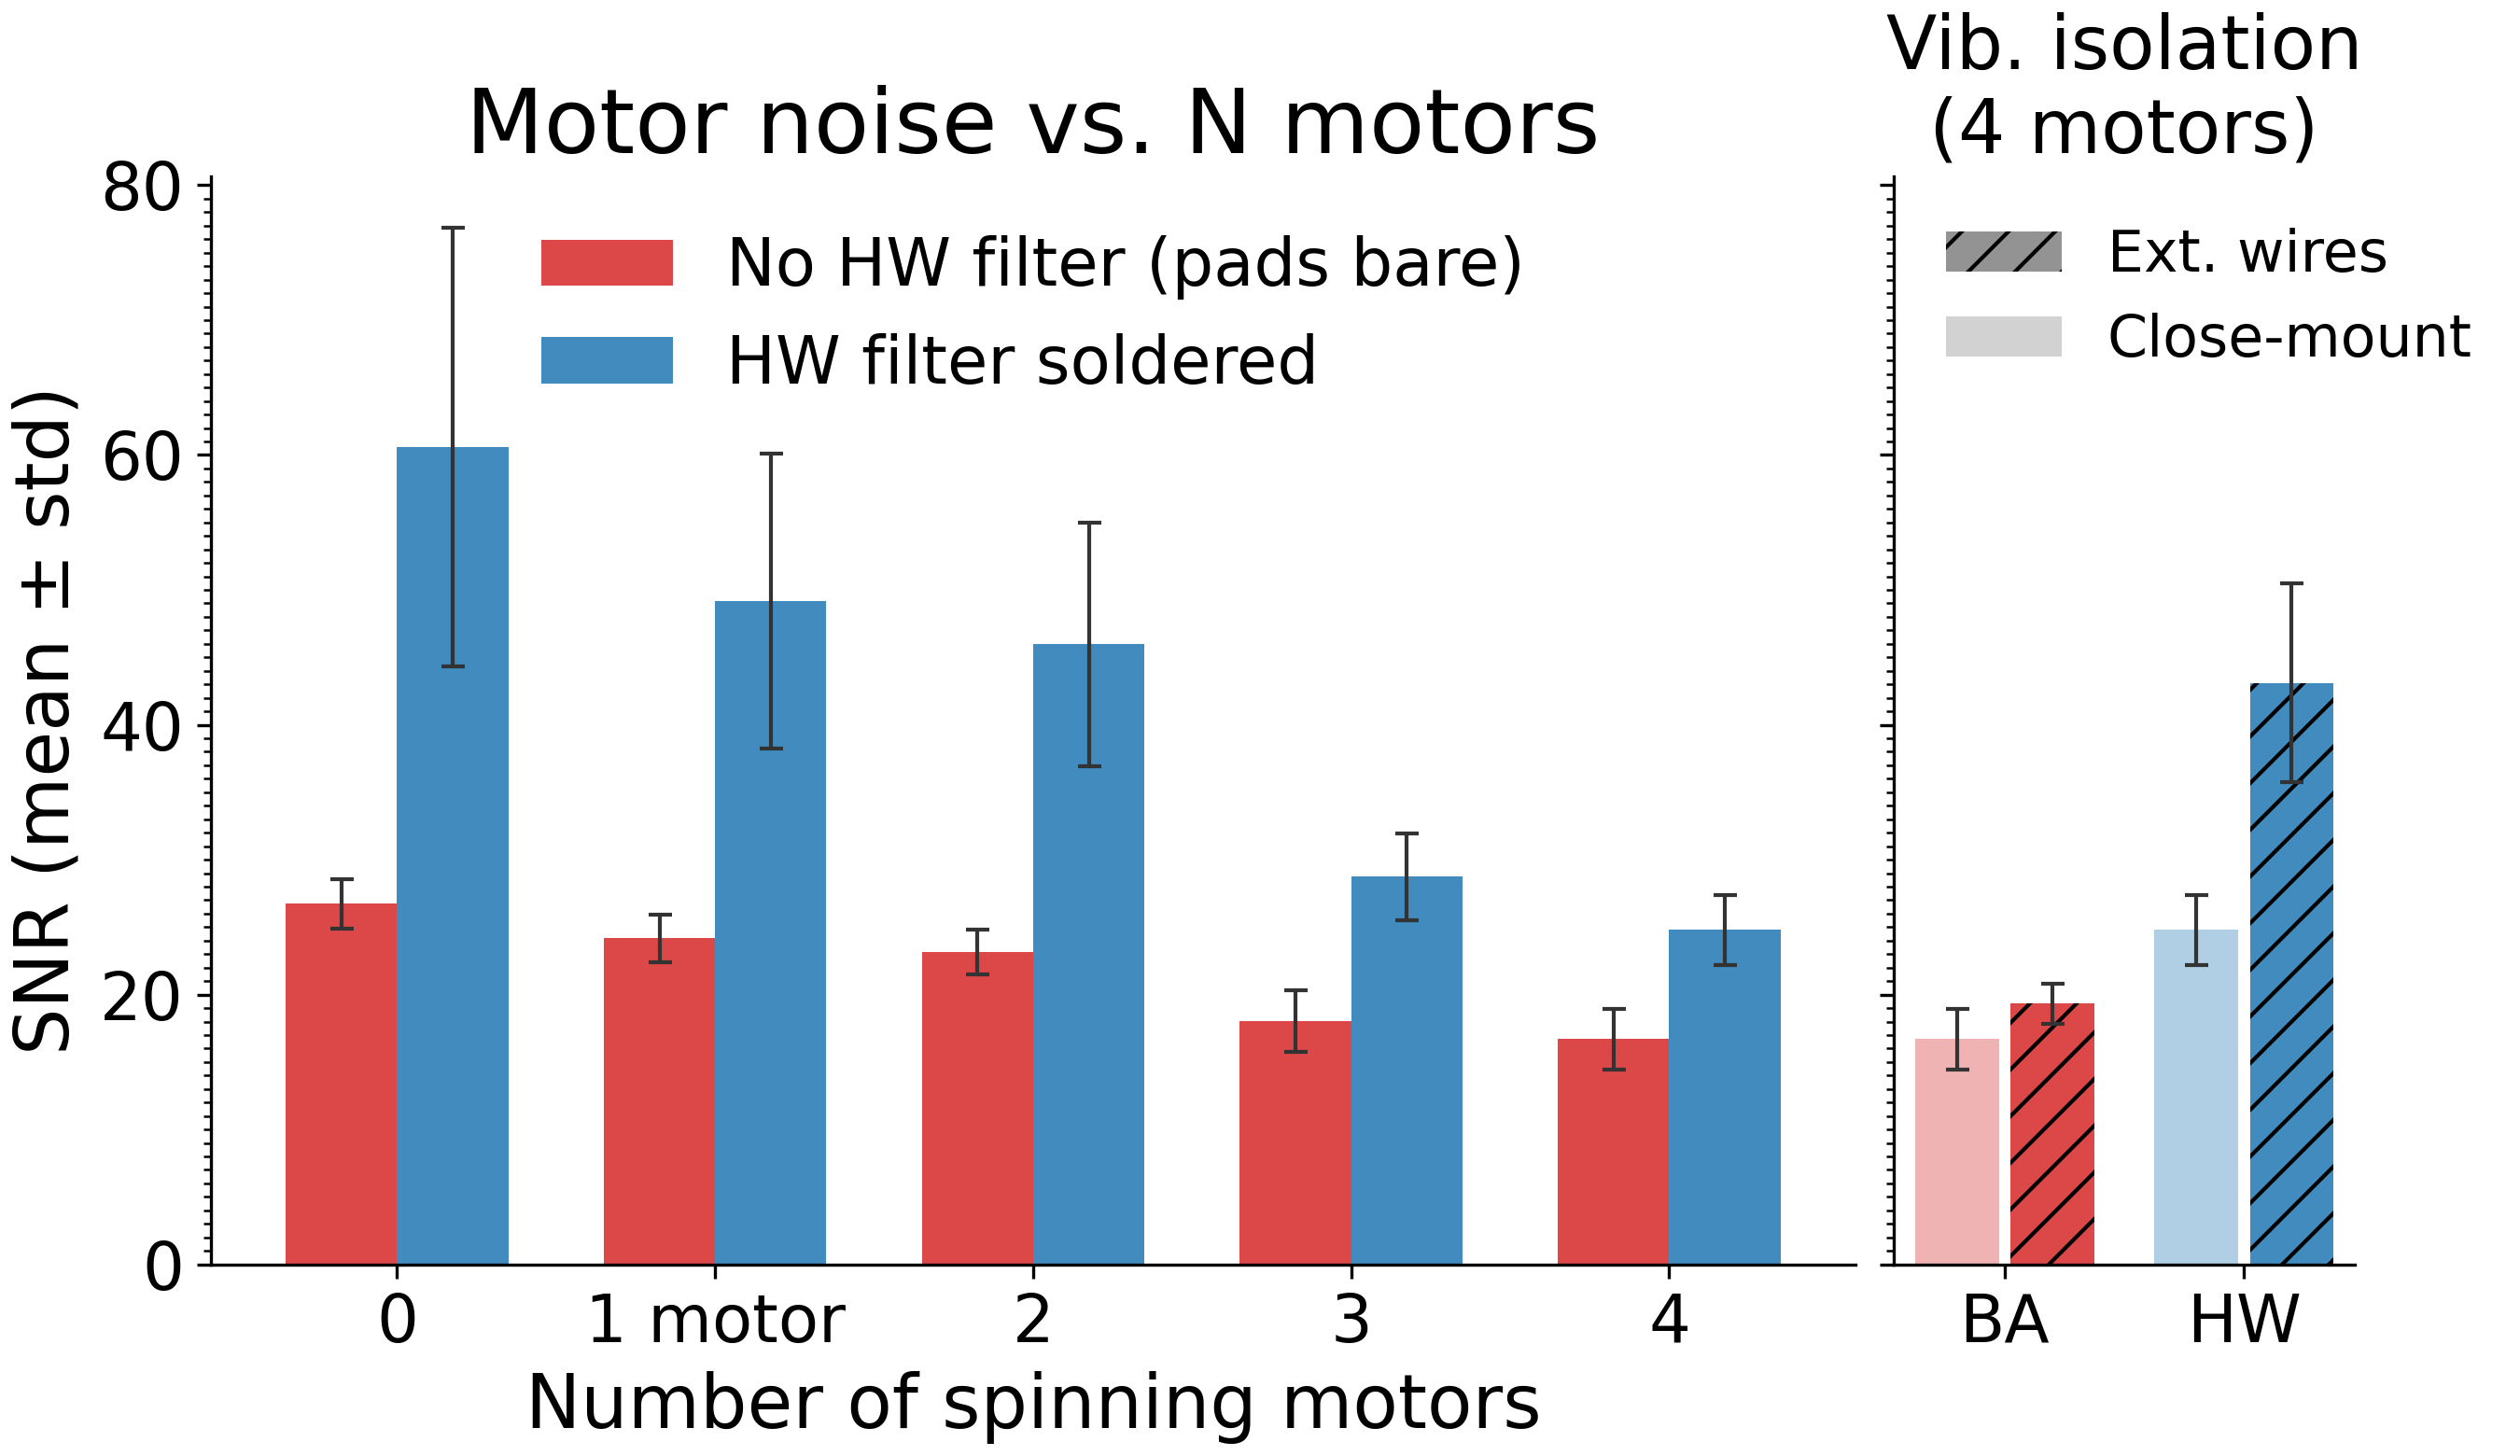
\includegraphics[width=0.85\textwidth]{figures/motor_noise.png}
    \caption{Overall SNR on the CrazyFlie as the number of running motors increases, with the hardware anti-alias filter unpopulated and soldered. The SNR falls as more motors spin, and the rightmost configuration moves the four motors onto extension wires to isolate their vibration from the board.}
    \label{fig:motor-noise}
\end{figure}\todo{The figure now contains BA and HW and are not explained. Please put explaination in the caption. }

This result\todo{What result?} connects back to the motivation of Chapter~\ref{chp:introduction}. The prior work we set out to extend could reach only a single beacon in open space, whereas the board and fused controller developed here now give that same platform the multi-beacon, obstacle-aware navigation it lacked.\todo{This paragraph feels misplaced. Almost as if it should be in the conclusion.}
